\section{Localization}

\subsection{IST}

\begin{figure}[H]
    \begin{subfigure}{0.45\textwidth}
        \centering
        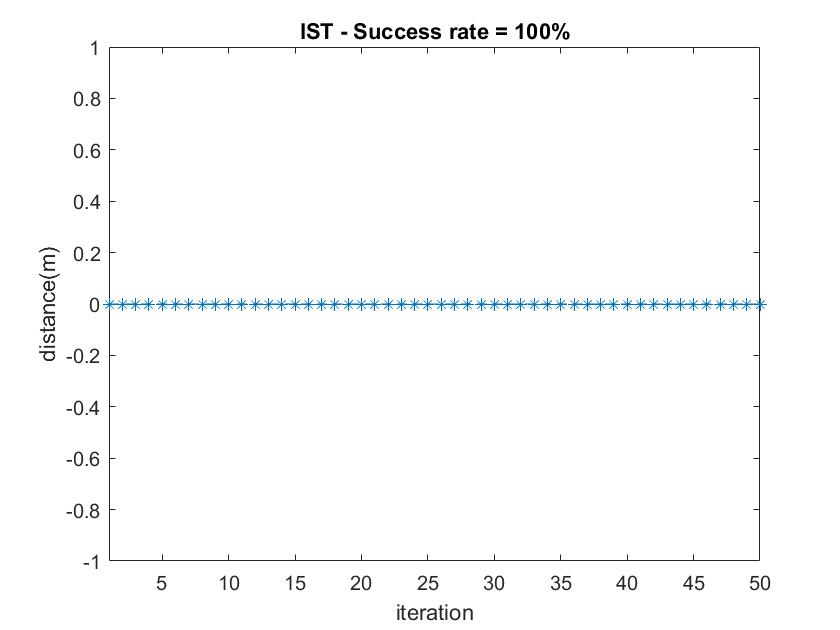
\includegraphics[width=\textwidth]{img/IST_distance_grid.jpg}
        \caption{Success rate of 100\%}
    \end{subfigure}
    \hfill
    \begin{subfigure}{0.45\textwidth}
        \centering
        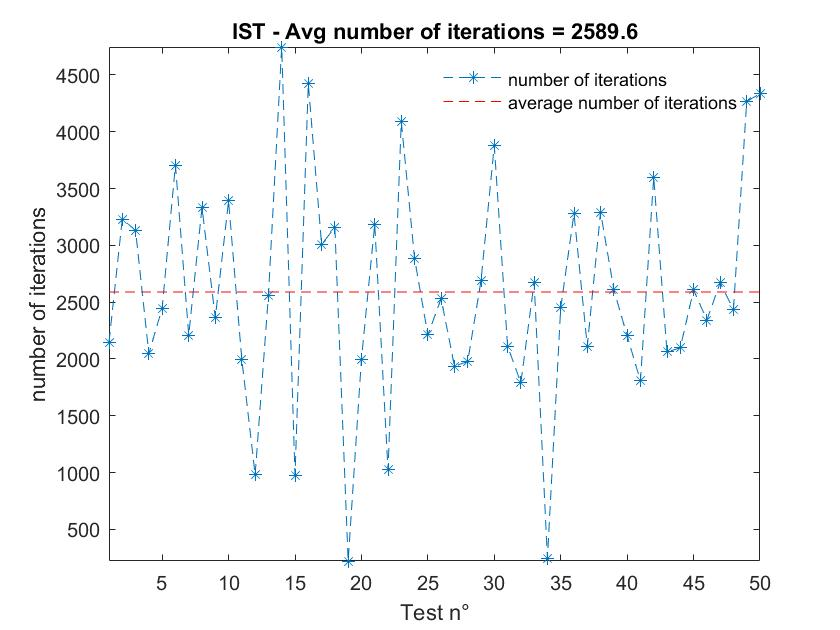
\includegraphics[width=\textwidth]{img/IST_num_iterations_grid.jpg}
        \caption{Average number of iterations}
    \end{subfigure}
    \caption{IST algorithm performed on grid topology ($\lambda=10^{-5},\,\tau=0.7,\,\epsilon=10^{-5}$)}
\end{figure}

We obtained a better accuracy with the grid topology because the room is uniformly covered by the sensors. By contrast, 
the uniform topology leaves some uncovered spaces, making the localization inaccurate: on average, the estimated
target is a cell adjacent to the correct one.\par
The average number of iterations is quite the same. In the uniform topology, the presence of errors increases the number of interations
to converge.

\begin{figure}[H]
    \begin{subfigure}{0.45\textwidth}
        \centering
        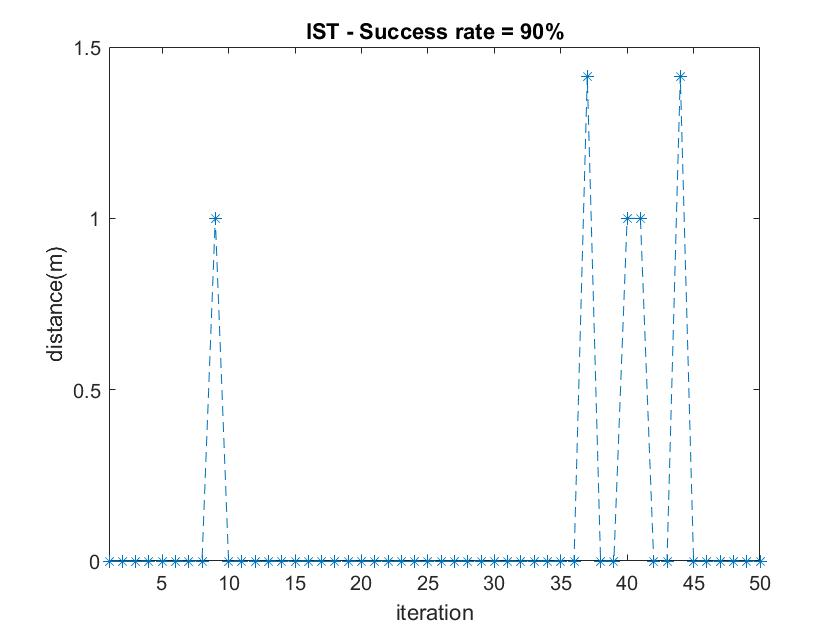
\includegraphics[width=\textwidth]{img/IST_distance_uniform.jpg}
        \caption{Success rate of 90\%}
    \end{subfigure}
    \hfill
    \begin{subfigure}{0.45\textwidth}
        \centering
        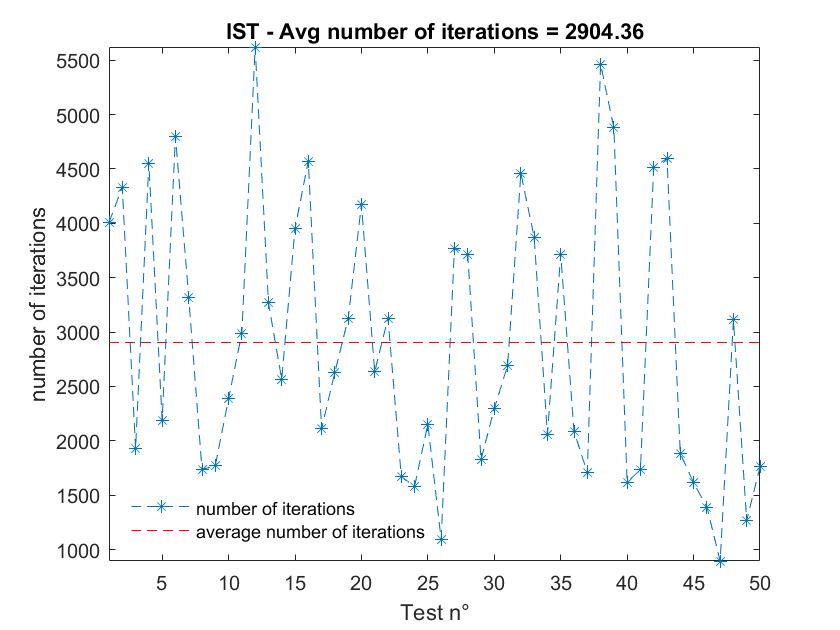
\includegraphics[width=\textwidth]{img/IST_num_iterations_uniform.jpg}
        \caption{Average number of iterations}
    \end{subfigure}
    \caption{IST algorithm performed on uniform topology ($\lambda=10^{-5},\,\tau=0.7,\,\epsilon=10^{-5}$)}
\end{figure}

\subsection{DIST}

With $\epsilon=10^{-5}$, the DIST algorithm performed on the grid topology stops , so we reduced it to $10^{-6}$, improving the accuracy
but, on the other hand, increasing the average number of iterations. Moreover, if we look at the results of 
the DIST algorithm with $\epsilon=10^{-5}$, we can notice that sensors have faster convergence time, but since we have to wait 
for the last sensor to converge, globally the number of iterations is bigger with respect to the IST algorithm.

\begin{figure}[H]
    \begin{subfigure}{0.45\textwidth}
        \centering
        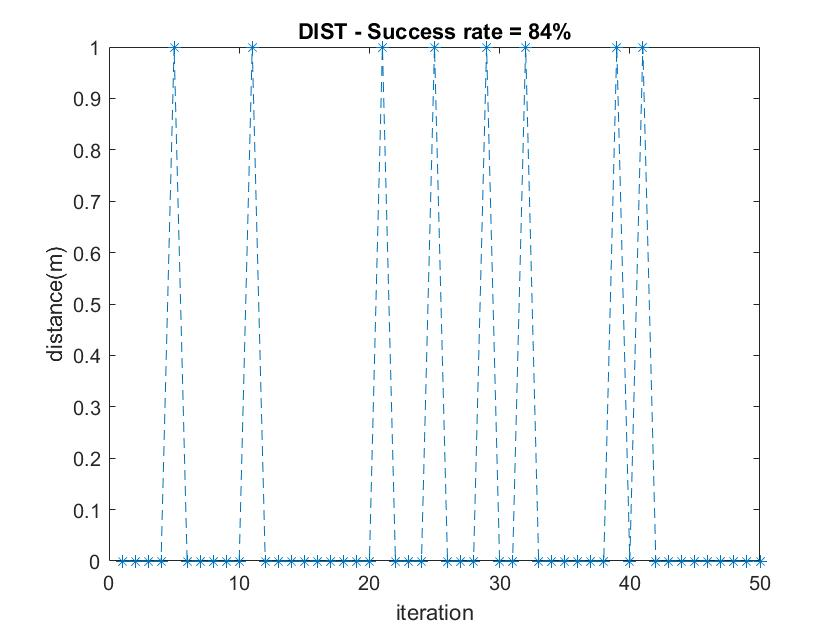
\includegraphics[width=\textwidth]{img/DIST_distance_1e-4_grid.jpg}
        \caption{Success rate of 84\%}
    \end{subfigure}
    \hfill
    \begin{subfigure}{0.45\textwidth}
        \centering
        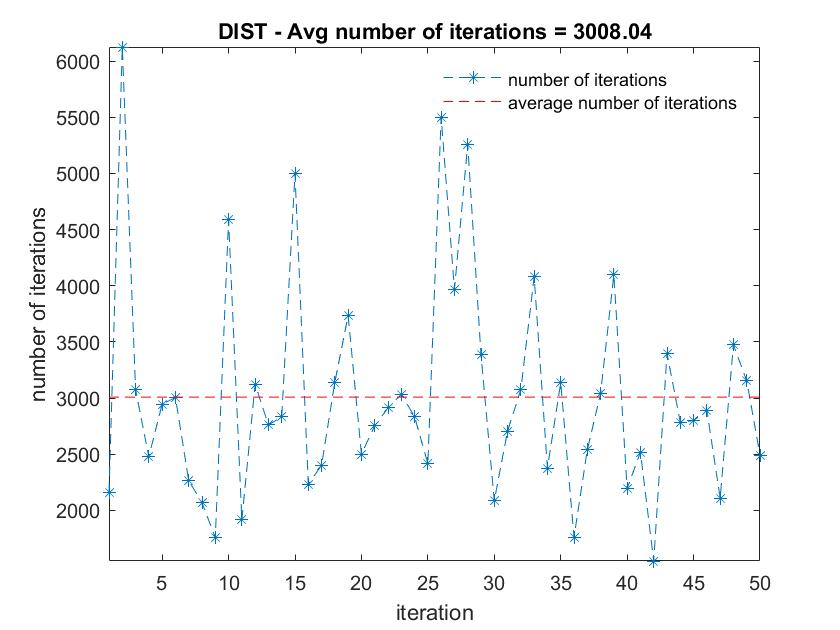
\includegraphics[width=\textwidth]{img/DIST_num_iterations_1e-4_grid.jpg}
        \caption{Average number of iterations}
    \end{subfigure}
    \caption{DIST algorithm performed on grid topology ($\lambda=10^{-5},\,\tau=0.7,\,\epsilon=10^{-5}$)}
\end{figure}
\begin{figure}[H]
    \begin{subfigure}{0.45\textwidth}
        \centering
        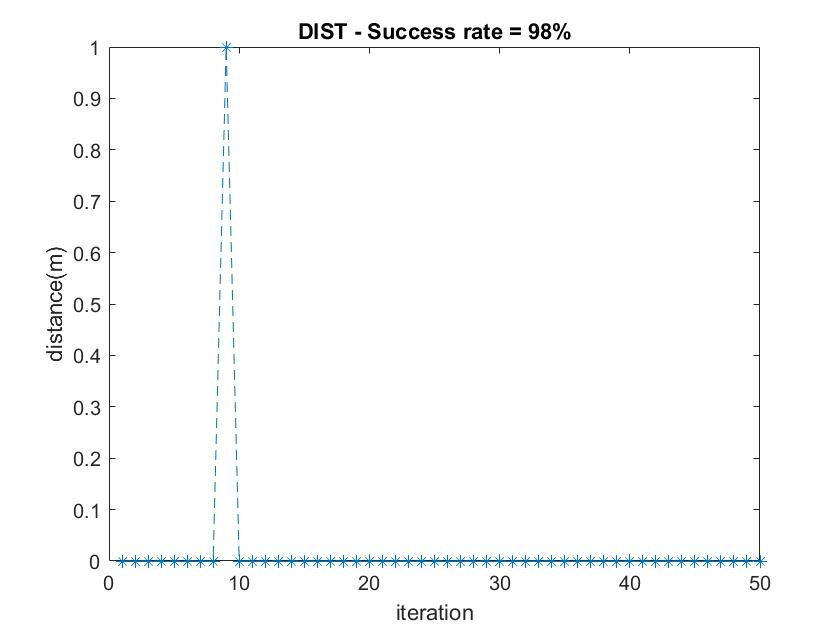
\includegraphics[width=\textwidth]{img/DIST_distance_1e-5_grid.jpg}
        \caption{Success rate of 98\%}
    \end{subfigure}
    \hfill
    \begin{subfigure}{0.45\textwidth}
        \centering
        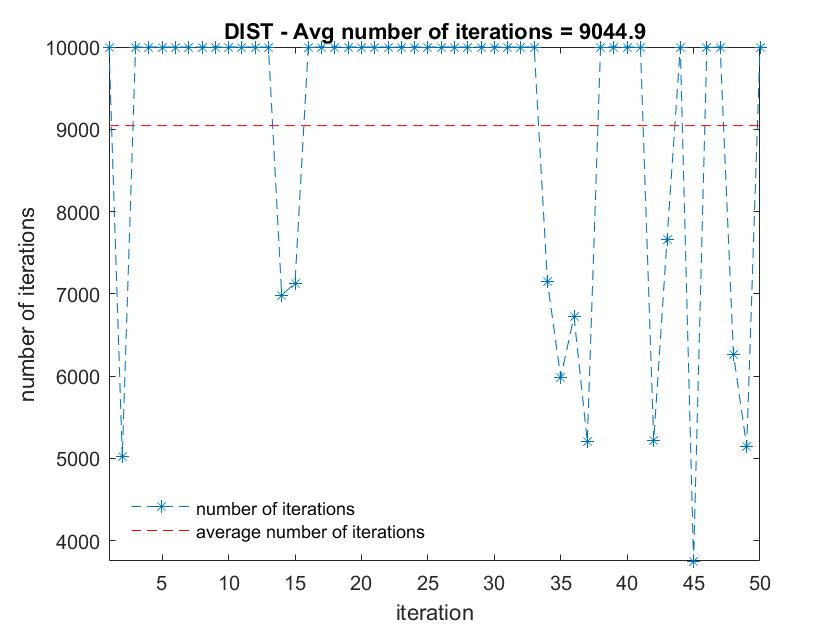
\includegraphics[width=\textwidth]{img/DIST_num_iterations_1e-5_grid.jpg}
        \caption{Average number of iterations}
    \end{subfigure}
    \caption{DIST algorithm performed on grid topology ($\lambda=10^{-5},\,\tau=0.7,\,\epsilon=10^{-6}$)}
\end{figure}

\begin{figure}[H]
    \begin{subfigure}{0.45\textwidth}
        \centering
        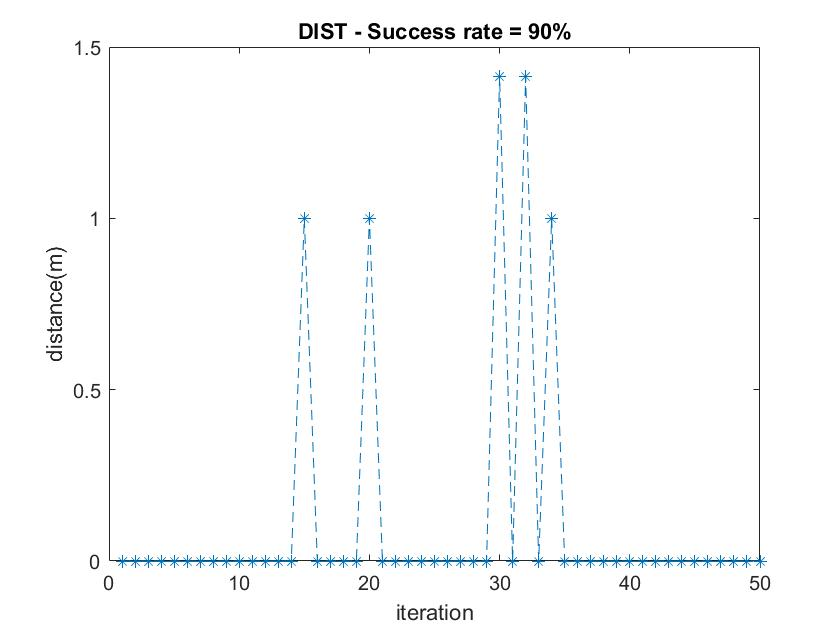
\includegraphics[width=\textwidth]{img/DIST_distance_uniform.jpg}
        \caption{Success rate of 90\%}
    \end{subfigure}
    \hfill
    \begin{subfigure}{0.45\textwidth}
        \centering
        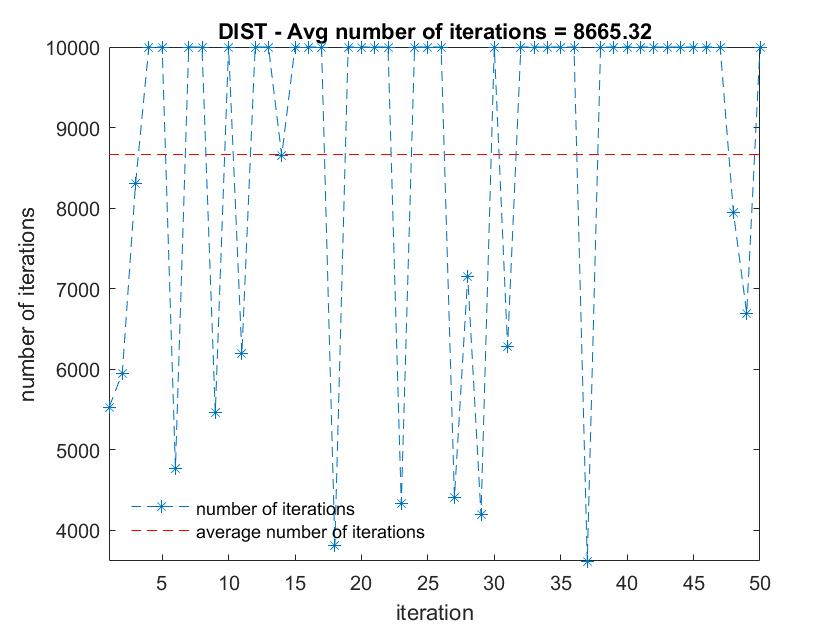
\includegraphics[width=\textwidth]{img/DIST_num_iterations_uniform.jpg}
        \caption{Average number of iterations}
    \end{subfigure}
    \caption{DIST algorithm performed on uniform topology ($\lambda=10^{-5},\,\tau=0.7,\,\epsilon=10^{-6}$)}
\end{figure}

As for the IST algorithm, we obtained a better accuracy with the grid topology but similar number of iterations.\par

After running multiple times the algorithm on different uniform topologies, we analyzed the convergence time with respect to the 
spectral radius of the matrix Q. As we can see from Figure \ref{fig: spectral radius analysis}, the number of iterations to achieve 
convergence grows with the spectral radius of the matrix Q.

\begin{figure}[H]
    \centering
    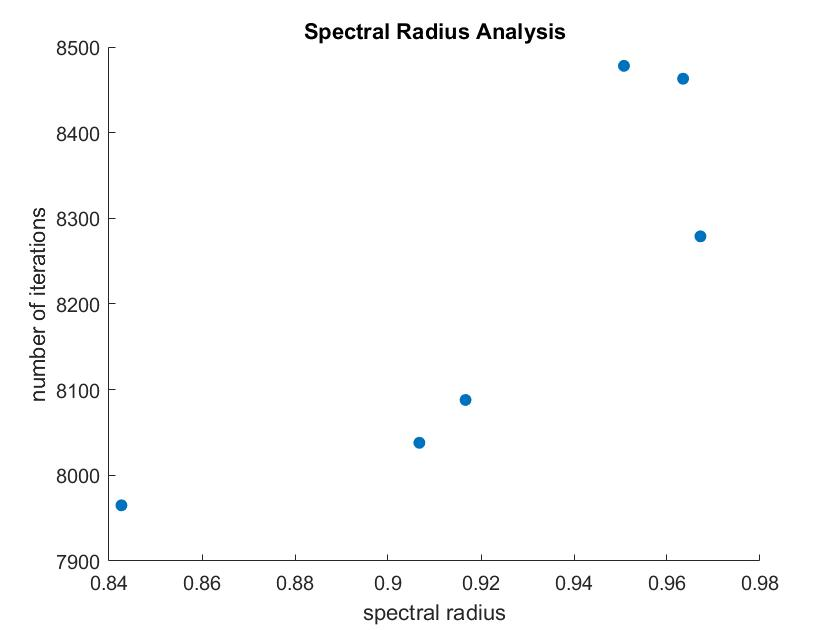
\includegraphics[width=.5\textwidth]{img/spectral_radius_analysis.jpg}
    \caption{Spectral Radius Analysis on uniform topology ($\lambda=10^{-5},\,\tau=0.7,\,\epsilon=10^{-6}$)}
    \label{fig: spectral radius analysis}
\end{figure}